\section{Evaluation}
\label{sec:evaluation}
This section presents our experiments with a case study of developing a software application for LEGO to evaluate the feasibility and usability of XSeparation.
The latter is implemented as an extension of the Papyrus modeling tool, which is based on Eclipse.
Architecture models in UML and XSeparation-generated C++ are synchronized.
Our XSeparation compiler supports POSIX systems, in which pthreads are used for concurrency in UML State Machines such as doActivity, parallel regions, and infinite loop for event dispatching.
The usage of C++11 standard threads can be easily integrated in the future.
For incremental code generation in XSeparation, a model listener based on IncQuery is hooked to the modeling tool to detect model modifications.

The additional constructs added to C++ are engineered in a way that allows programmers to use facilities such as auto-completion of any C++ IDE to write interaction code between components or state machine descriptions.
It means that the programmers can stay within their familiar IDE and its facilities to effectively write code.
This is one of our advantages over other approaches which will be discussed in Section \ref{sec:relatedwork}. 
For example, Fig. \ref{fig:autocompletion} shows auto-completions for writing interaction codes for the examples in case using interface and data ports within Eclipse CDT ((a) and (b)) and Visual Studio ((c) and (d)).
Note that no additional tools need to be installed for the auto-completions.

\begin{figure}
	\centering
	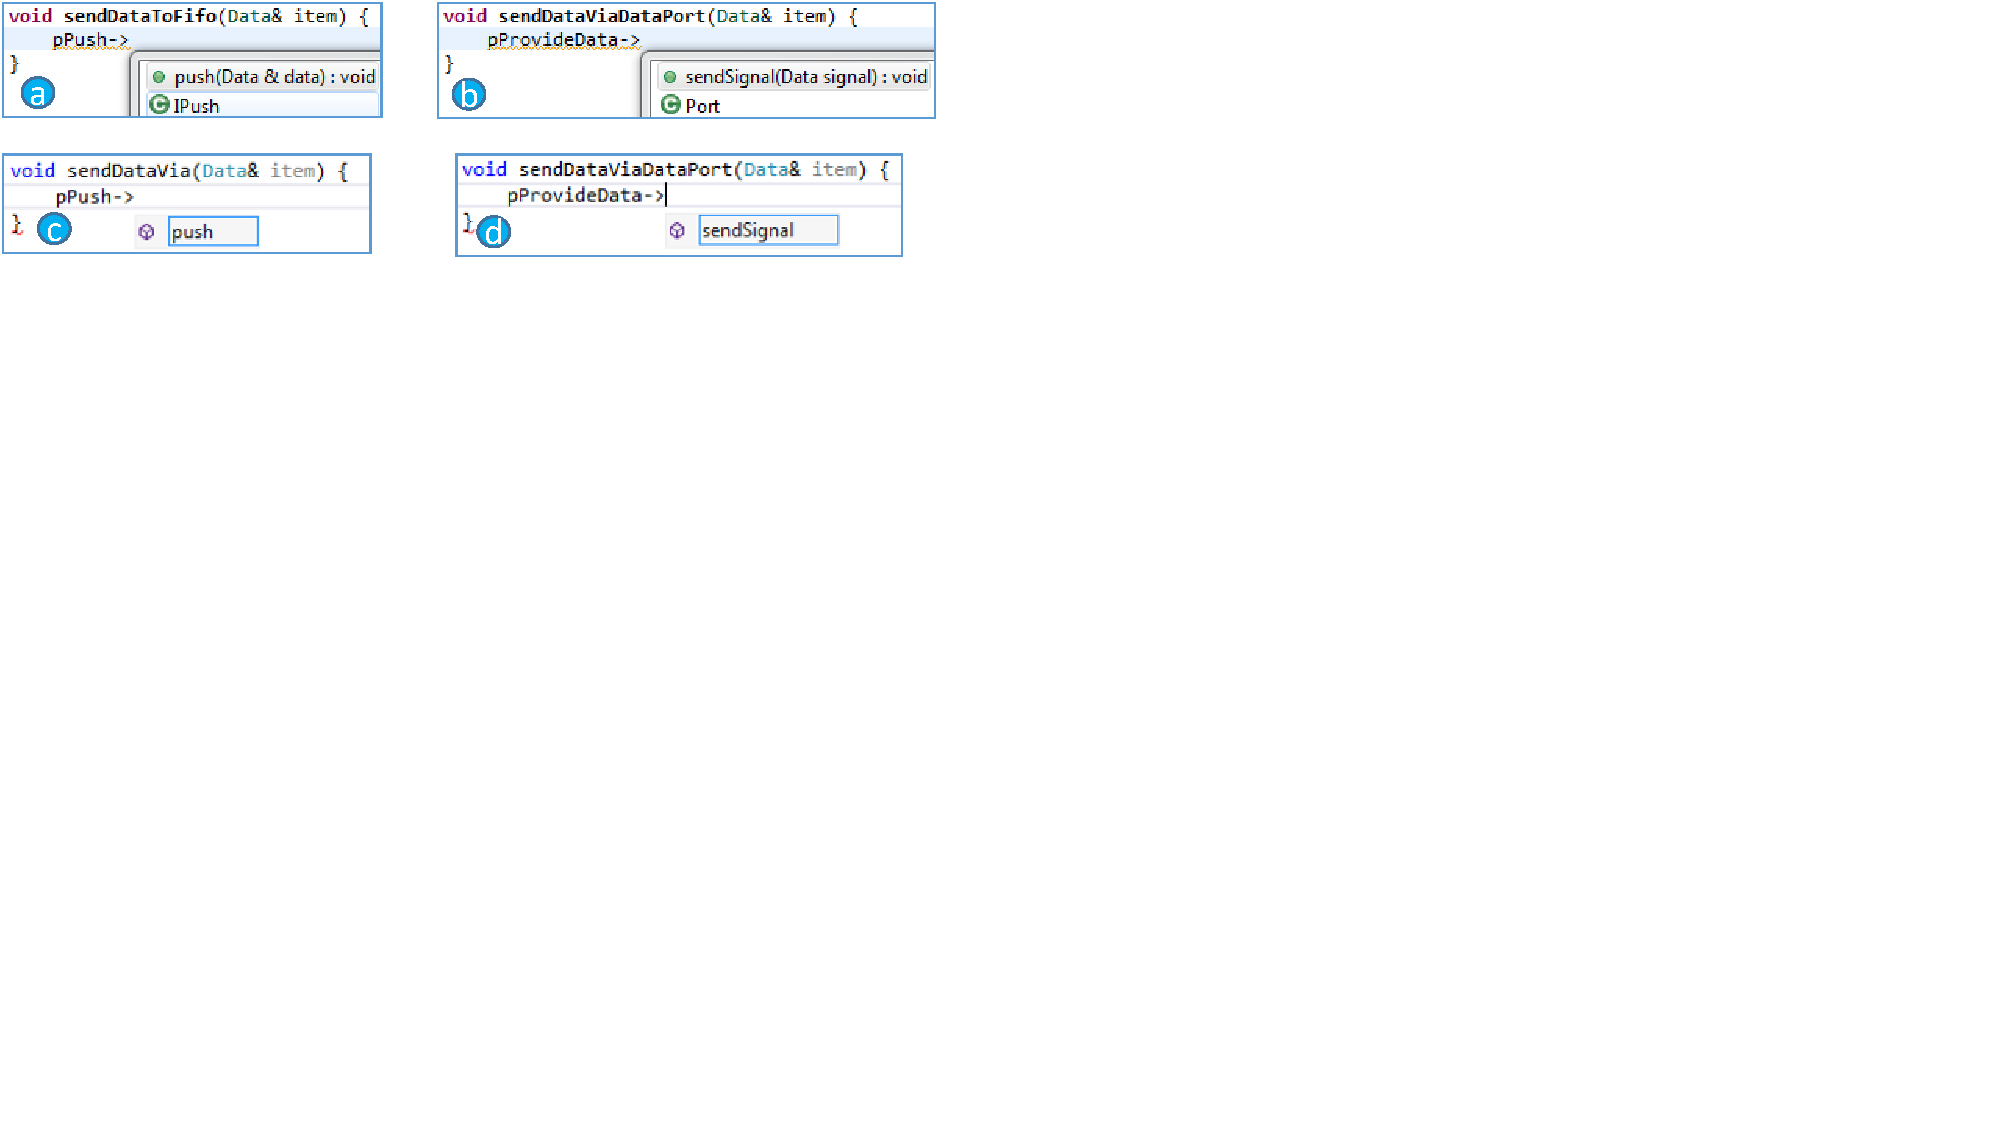
\includegraphics[clip, trim=0cm 14.6cm 17.7cm 0cm, width=\columnwidth]{figures/autocompletion.pdf}
	\caption{Auto-completions for XSeparation-generated code from the examples with interface and data ports: (a) and (b) in CDT and (c) and (d) in Visual Studio} 
	\label{fig:autocompletion}
\end{figure}

After implementation, we then developed a software application for LEGO in order to evaluate XSeparation through the tooling prototype.
The followings present the case study development for the applicability evaluation and a manual evaluation of the usability.
%\subsection{Implementation}

\subsection{Case study development}
Description of the application...

The case study was developed by a developer \tb{Dev}. 
\tb{Dev} used the Papyrus Designer tool, which features component-based and model-driven development in UML and full C++ code generation through embedding of fine-grained code as blocks of texts within a limited text editor.   

During the development, an architecture model is created.
However, the developer felt difficult, unfamiliar, and annoyed to write code with the limited editor.
\tb{Dev} then refused to use that editor and programmed in CDT to be familiar and effective with C++ facilities such as syntax highlights and auto-completion.
\tb{Dev} then copied the code from CDT to the model and regenerated the code.
The developer felt inefficient, prone-to-error, and lack comprehension of the architecture information during code writing and copying.

Given the above issues, \tb{Dev} wants to try a synchronization approach, which at least can automatically synchronize modifications in fine-grained behavior to the model.

\vskip 0.1cm
\noindent
\tb{Application of XSeparation}:
We applied XSeparation to two distinct scenarios: (1) \tb{Dev} modifies both model and code; and (2) A collaboration scenario between \tb{Dev}, as a programmer, and a software architect. 

\vskip 0.1cm
\noindent
\tb{Scenario 1}:
In this scenario, \tb{Dev} managed the application revision by using Git.
\tb{Dev} used Papyrus Designer to create the architecture model, and generates intermediate and executable code from it.
She then filled fine-grained behavior in the intermediate code using CDT.
After that, \tb{Dev} then used XSeparation to regenerate the executable code and compiled it.
The modified intermediate code is then automatically synchronized back to the original architecture model by using XSeparation.
Following each synchronization, \tb{Dev} committed and pushed both of the model, the intermediate code, and the executable code to Git.  

\vskip 0.1cm
\noindent
\tb{Scenario 2}:
\tb{Dev} and an other developer \tb{OtherDev} use Git to control versions of the case study project and work together.
In the beginning, the component-based architecture structure model is created by the two developers using Papyrus Designer.
Intermediate and executable code are then generated from the model by XSeparation.
The model and codes are then pushed to the Git repository as an initial version.
Each developer took in charge of development of several components.
For each corresponding component, each of the developers then described its course-grained behavior via a UML State machine, regenerated the intermediate code, wrote fine-grained code for the component, and synchronized the modified intermediate code with the model by using XSeparation.
After synchronization, the developer tried to pulled the artifacts from the remote Git repository.
If the remote model was updated by the other developer, both of the models were merged with each other using the Papyrus model merger \cite{collaborativepapyrus}.
After merging, the intermediate code is then regenerated.
The two artifacts are then pushed to the remote repository.
  


%\subsection{Evaluations of Incremental code generation and reverse engineering in XSeparation}

\subsection{Usability evaluation}
To evaluate the usability of XSeparation, several questions are used for asking developers for how effective XSeparation is when compared to full code generation approaches using fine-grained code directly embedded within models.

\paragraph{Is model-code synchronization in XSeparation better than full code generation with fine-grained code within models in general?}

\paragraph{Is modifying architecture at the code level more effective than at the model level?}

\paragraph{Is modifying fine-grained code at the code level better than code embedded within models for full code generation?}

\paragraph{Is concurrent development using XSeparation effective?}

\lipsum[1-2]
